
\documentclass[12pt]{article} % use larger type; default would be 10pt
\usepackage[square]{natbib}
\usepackage[utf8]{inputenc} % set input encoding (not needed with XeLaTeX)
\usepackage{amsmath,amssymb}
\DeclareMathOperator{\E}{\mathbb{E}}
\usepackage{color}
\usepackage{pdfpages}
%%% PAGE DIMENSIONS
\usepackage{geometry} % to change the page dimensions
\geometry{a4paper} % or letterpaper (US) or a5paper or....
 \geometry{margin=1in} % for example, change the margins to 2 inches all round
% \geometry{landscape} % set up the page for landscape
%   read geometry.pdf for detailed page layout information
 \newcommand{\eps}{\varepsilon}
\usepackage{graphicx} % support the \includegraphics command and options

% \usepackage[parfill]{parskip} % Activate to begin paragraphs with an empty line rather than an indent

%%% PACKAGES
\usepackage{booktabs} % for much better looking tables
\usepackage{array} % for better arrays (eg matrices) in maths
\usepackage{paralist} % very flexible & customisable lists (eg. enumerate/itemize, etc.)
\usepackage{verbatim} % adds environment for commenting out blocks of text & for better verbatim
\usepackage{subfig} % make it possible to include more than one captioned figure/table in a single float
% These packages are all incorporated in the memoir class to one degree or another...

%%% HEADERS & FOOTERS
\usepackage{fancyhdr} % This should be set AFTER setting up the page geometry
%\pagestyle{fancy} % options: empty , plain , fancy

\usepackage{tikz}

\fancypagestyle{firstpage}
{
\renewcommand{\headrulewidth}{1pt} % customise the layout...
\lhead{STAT 400 (FA26)}\chead{HW 06}\rhead{}
\lfoot{}\cfoot{\thepage}\rfoot{}
}


%%% SECTION TITLE APPEARANCE
\usepackage{sectsty}
\allsectionsfont{\sffamily\mdseries\upshape} % (See the fntguide.pdf for font help)
% (This matches ConTeXt defaults)

%%% ToC (table of contents) APPEARANCE
\usepackage[nottoc,notlof,notlot]{tocbibind} % Put the bibliography in the ToC
\usepackage[titles,subfigure]{tocloft} % Alter the style of the Table of Contents
\renewcommand{\cftsecfont}{\rmfamily\mdseries\upshape}
\renewcommand{\cftsecpagefont}{\rmfamily\mdseries\upshape} % No bold!


\definecolor{Red}{rgb}{1,0,0}
\newcommand{\Red}{\color{Red}}
\definecolor{Blue}{rgb}{0,0,1}
\newcommand{\Blue}{\color{Blue}}


%%%%%%%THEOREM 
\usepackage{thmtools,thm-restate}
\newtheorem{theorem}{Theorem}
\newtheorem{lemma}[theorem]{Lemma}
\newtheorem{proposition}[theorem]{Proposition}
\newtheorem{corollary}[theorem]{Corollary}

\newenvironment{proof}[1][Proof]{\begin{trivlist}
\item[\hskip \labelsep {\bfseries #1}]}{\end{trivlist}}
\newenvironment{definition}[1][Definition]{\begin{trivlist}
\item[\hskip \labelsep {\bfseries #1}]}{\end{trivlist}}
\newenvironment{example}[1][Example]{\begin{trivlist}
\item[\hskip \labelsep {\bfseries #1}]}{\end{trivlist}}
\newenvironment{remark}[1][Remark]{\begin{trivlist}
\item[\hskip \labelsep {\bfseries #1}]}{\end{trivlist}}

\newcommand{\qed}{\nobreak \ifvmode \relax \else
      \ifdim\lastskip<1.5em \hskip-\lastskip
      \hskip1.5em plus0em minus0.5em \fi \nobreak
      \vrule height0.75em width0.5em depth0.25em\fi}
   
     \usepackage{tikz}
  \def\firstcircle{(90:1cm) circle (1.5cm)}
  \def\secondcircle{(210:1cm) circle (1.5cm)}
  \def\thirdcircle{(330:1cm) circle (1.5cm)}
   
   
%\usepackage{nopageno}   
 %%%%%%%%%%%%%%

\linespread{2}


\usepackage{enumitem}



%%% END Article customizations



%%% The "real" document content comes below...






\begin{document}
%\maketitle
\thispagestyle{firstpage}


\begin{enumerate}

\item Amy and Janet have agreed to meet for lunch between noon and 1pm. Denote Janet's arrival time by $X$ and Amy's by $Y$, and suppose $X$ and $Y$ are independent with probability density functions
	\begin{equation*}
			f_{X}(x)=\begin{cases}
			3x^2,  & 0\leq x\leq 1\\
			0 & \text{otherwise}
			\end{cases}, 
			\quad
				f_{Y}(y)=\begin{cases}
			2y,  & 0\leq y\leq 1\\
			0 & \text{otherwise}
			\end{cases}, 
	\end{equation*}
Find the probability that Janet arrives before Amy. That is, find $P(X<Y)$. \\ {\Red $$\begin{aligned}
    P(X < Y) &= \int \int_{\{x < y\}} f(x) f(y) dxdy \\
    &= \int_0^1 \int_0^y 6x^2y dxdy \\
    &=\int_0^1 y \int_0^y 6x^2 dxdy \\
    &= \int_0^1 y \Big[ 2x^3\Big]_0^y dy \\
    &= \int_0^1 2y^4 dy \\
    &= \frac{2}{5} y^5 \Bigg \vert_{0}^1 \\
    &= 0.4
\end{aligned}$$}
\newpage
\item Suppose that the random variables $X$ and $Y$ have joint pdf given by
	\begin{equation*}
			f(x,y)=\begin{cases}
			Cx^2 y ,&0<x<y,\quad x+y<2,\\
			0 & \text{otherwise}.
			\end{cases}
	\end{equation*}
	\begin{enumerate}[label=2.\arabic*]
		\item[] Let's draw the area of the support of $(X,Y)$.
        {\Red
        \begin{align*}
        f(x,y)>0 \iff 0<x<y,\quad x+y<2.
        \end{align*}
        Equivalently,
        \begin{align*}
        0<x<1,\qquad x<y<2-x.
        \end{align*}
        \begin{center}
        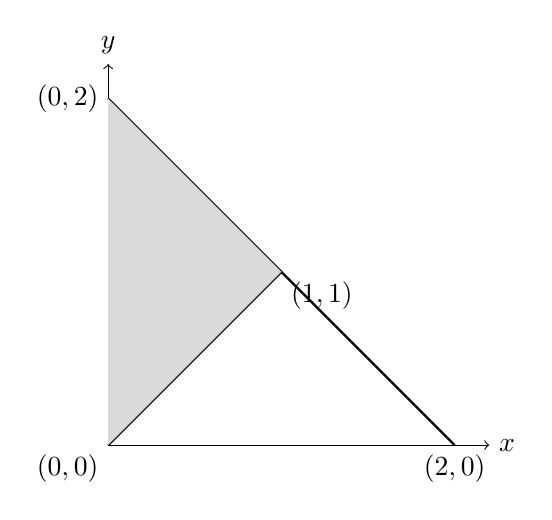
\begin{tikzpicture}[scale=2.2]
        \draw[->] (0,0) -- (2.2,0) node[right] {$x$};
        \draw[->] (0,0) -- (0,2.2) node[above] {$y$};
        \draw[thick] (0,0) -- (1,1);
        \draw[thick] (0,2) -- (2,0);
        \fill[gray!30] (0,0) -- (0,2) -- (1,1) -- cycle;
        \node at (1,1) [below right] {$(1,1)$};
        \node at (0,2) [left] {$(0,2)$};
        \node at (2,0) [below] {$(2,0)$};
        \node at (0,0) [below left] {$(0,0)$};
        \end{tikzpicture}
        \end{center}
        }
		\item What must be the value of $C$ so that $f(x,y)$ is a valid joint pdf?
        {\Red
        \begin{align*}
        1&=\int_{0}^{1}\int_{y=x}^{2-x} Cx^2ydydx \\
        &=\int_{0}^{1} Cx^2\left[\frac{y^2}{2}\right]_{x}^{2-x} dx \\
        &=\int_{0}^{1} Cx^2\cdot \frac{(2-x)^2-x^2}{2} dx \\
        &=\int_{0}^{1} Cx^2(2-2x) dx \\
        &=2C\int_{0}^{1}(x^2-x^3) dx
        =2C\left(\frac13-\frac14\right)
        =\frac{C}{6}.
        \end{align*}
        \begin{align*}
        \Rightarrow\quad C=6.
        \end{align*}
        }
		\item Find $P(X+Y<1)$.\\
        {\Red
        On the event $X+Y<1$ with $0<X<Y$, we have $X<\tfrac12$.
        \begin{align*}
        P(X+Y<1)&=\int_{0}^{1/2}\int_{y=x}^{1-x} 6x^2ydydx \\
        &=\int_{0}^{1/2} 6x^2\left[\frac{y^2}{2}\right]_{x}^{1-x}dx \\
        &=\int_{0}^{1/2} 3x^2\big((1-x)^2-x^2\big)dx \\
        &=\int_{0}^{1/2} 3x^2(1-2x)dx\\
        &=3\left[\frac{x^3}{3}-\frac{x^4}{2}\right]_{0}^{1/2}\\
        &=\frac{1}{32}.
        \end{align*}

        }
		\item Find the marginal probability density function for $X$. Include the support.
        {\Red
        For $0<x<1$, we have $x<y<2-x$:
        \begin{align*}
        f_X(x)&=\int_{x}^{2-x} 6x^2ydy
        =6x^2\left[\frac{y^2}{2}\right]_{x}^{2-x}
        =6x^2(2-2x)
        =12x^2(1-x).
        \end{align*}
        \begin{align*}
        f_X(x)=
        \begin{cases}
        12x^2(1-x), & 0<x<1,\\
        0, & \text{otherwise}.
        \end{cases}
        \end{align*}
        }
		\item[] Find the marginal probability density function for $Y$. Include the support. (This was not asked in HW, but necessary for the next step)\\
        {\Red
        For fixed $y$:
        \begin{align*}
         0<x<\min(y,2-y).
        \end{align*}
        Thus
        \begin{align*}
        f_Y(y)
        &=\int_{0}^{\min(y,2-y)} 6x^2ydx
        =6y\left[\frac{x^3}{3}\right]_{0}^{\min(y,2-y)}
        =2y\big(\min(y,2-y)\big)^3.
        \end{align*}
        So
        \begin{align*}
        f_Y(y)=
        \begin{cases}
        2y^4, & 0<y<1,\\
        2y(2-y)^3, & 1<y<2,\\
        0, & \text{otherwise}.
        \end{cases}
        \end{align*}
        }
		\item Are $X$ and $Y$ independent? Why or why not? 
        {\Red
        \begin{align*}
        f(x,y)\neq f_X(x)f_Y(y).
        \end{align*}
        Therefore $X$ and $Y$ are not independent.
        }
		\item Find the Covariance of $X$ and $Y$. 
        {\Red
        \begin{align*}
        \operatorname{Cov}(X,Y)
        &=\mathbb E[XY]-\mathbb E[X]\mathbb E[Y].
        \end{align*}
        \begin{align*}
        \mathbb E[X]
        &=\int_{0}^{1}\int_{x}^{2-x} x\cdot 6x^2y dy dx
        = \frac{3}{5},\\[6pt]
        \mathbb E[Y]
        &=\int_{0}^{1}\int_{x}^{2-x} y\cdot 6x^2y dy dx
        = \frac{16}{15},\\[6pt]
        \mathbb E[XY]
        &=\int_{0}^{1}\int_{x}^{2-x} xy\cdot 6x^2y dy dx
        = \frac{22}{35}.
        \end{align*}
        \begin{align*}
        \operatorname{Cov}(X,Y)
        &=\frac{22}{35}-\left(\frac{3}{5}\right)\left(\frac{16}{15}\right)
        =\frac{22}{35}-\frac{16}{25}
        =-\frac{2}{175}.
        \end{align*}
        }
		%\item Find the Correlation coefficient of $X$ and $Y$.
	\end{enumerate}
\newpage
\item Suppose that the random variables $X$ and $Y$ have joint pdf given by
	\begin{equation*}
			f(x,y)=\begin{cases}
			x+4y , & 0<y<x<1,\\
			0 & \text{otherwise}.
			\end{cases}
	\end{equation*}

Find $P(X>4Y)$.

 {\Red
        \begin{align*}
        f(x,y)>0 &\iff 0<y<x<1.
        \end{align*}
        Hence the support is
        \begin{align*}
        \{(x,y): 0<y<x<1\},
        \end{align*}
        a triangular region below $y=x$, above $y=0$, and left of $x=1$.
        \begin{center}
        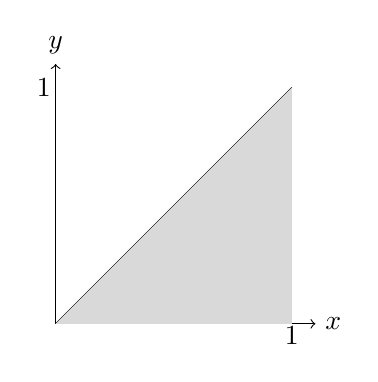
\begin{tikzpicture}[scale=3]
        \draw[->] (0,0) -- (1.1,0) node[right] {$x$};
        \draw[->] (0,0) -- (0,1.1) node[above] {$y$};
        \draw (0,0) -- (1,0);
        \draw (1,0) -- (1,1);
        \draw (0,0) -- (1,1);
        
        \fill[gray!30] (0,0) -- (1,0) -- (1,1) -- cycle;    
        \node at (1,-0.05) {$1$};
        \node at (-0.05,1) {$1$};
        \end{tikzpicture}
        \end{center}
        }

        {\Red
        \begin{align*}
        X>4Y 
        &\iff Y<\frac{X}{4}.
        \end{align*}
        Since $\frac{x}{4}<x$ for $0<x<1$,
        \begin{align*}
        P(X>4Y)
        &=\int_{0}^{1}\int_{0}^{x/4}(x+4y)dydx.
        \end{align*}
        Compute the inner integral:
        \begin{align*}
        \int_{0}^{x/4}(x+4y)dy=\left[xy+2y^2\right]_{0}^{x/4} =\frac{x^2}{4}+\frac{x^2}{8} =\frac{3x^2}{8}.
        \end{align*}
        Therefore,
        \begin{align*}
        P(X>4Y)=\int_{0}^{1}\frac{3x^2}{8}dx =\frac{3}{8}\cdot\frac{1}{3} =\frac18.
        \end{align*}
        }
    
	% \begin{enumerate}[label=3.\arabic*]
	% 	\item[] Draw the area of the support of $(X,Y)$.
 %        {\Red
 %        \begin{align*}
 %        f(x,y)>0 &\iff 0<y<x<1.
 %        \end{align*}
 %        Hence the support is
 %        \begin{align*}
 %        \{(x,y): 0<y<x<1\},
 %        \end{align*}
 %        a triangular region below $y=x$, above $y=0$, and left of $x=1$.
 %        \begin{center}
 %        \begin{tikzpicture}[scale=3]
 %        \draw[->] (0,0) -- (1.1,0) node[right] {$x$};
 %        \draw[->] (0,0) -- (0,1.1) node[above] {$y$};
 %        \draw (0,0) -- (1,0);
 %        \draw (1,0) -- (1,1);
 %        \draw (0,0) -- (1,1);
        
 %        \fill[gray!30] (0,0) -- (1,0) -- (1,1) -- cycle;    
 %        \node at (1,-0.05) {$1$};
 %        \node at (-0.05,1) {$1$};
 %        \end{tikzpicture}
 %        \end{center}
 %        }
	% 	\item Find $P(X>4Y)$.
 %        {\Red
 %        \begin{align*}
 %        X>4Y 
 %        &\iff Y<\frac{X}{4}.
 %        \end{align*}
 %        Since $\frac{x}{4}<x$ for $0<x<1$,
 %        \begin{align*}
 %        P(X>4Y)
 %        &=\int_{0}^{1}\int_{0}^{x/4}(x+4y)dydx.
 %        \end{align*}
 %        Compute the inner integral:
 %        \begin{align*}
 %        \int_{0}^{x/4}(x+4y)dy=\left[xy+2y^2\right]_{0}^{x/4} =\frac{x^2}{4}+\frac{x^2}{8} =\frac{3x^2}{8}.
 %        \end{align*}
 %        Therefore,
 %        \begin{align*}
 %        P(X>4Y)=\int_{0}^{1}\frac{3x^2}{8}dx =\frac{3}{8}\cdot\frac{1}{3} =\frac18.
 %        \end{align*}
 %        }
	% 	\item Find the marginal probability density function for $X$. Include the support.
 %        {\Red
 %        For $0<x<1$,
 %        \begin{align*}
 %        f_X(x)=\int_{0}^{x}(x+4y)dy =\left[xy+2y^2\right]_{0}^{x} =x^2+2x^2 =3x^2.
 %        \end{align*}
 %        Thus
 %        \begin{align*}
 %        f_X(x)=
 %        \begin{cases}
 %        3x^2, & 0<x<1,\\
 %        0, & \text{otherwise}.
 %        \end{cases}
 %        \end{align*}
 %        }
	% 	\item[] Find the marginal probability density function for $Y$. Include the support. (This part was not asked directly in the HW, but necessary for the next step)
 %        {\Red
 %        For $0<y<1$,
 %        \begin{align*}
 %        f_Y(y)=\int_{y}^{1}(x+4y)dx =\left[\frac{x^2}{2}+4yx\right]_{y}^{1} =\left(\frac12+4y\right)-\left(\frac{y^2}{2}+4y^2\right) =\frac12+4y-\frac{9}{2}y^2.
 %        \end{align*}
 %        Thus
 %        \begin{align*}
 %        f_Y(y)=
 %        \begin{cases}
 %        \frac12+4y-\frac{9}{2}y^2, & 0<y<1,\\
 %        0, & \text{otherwise}.
 %        \end{cases}
 %        \end{align*}
 %        }
	% 	\item Are $X$ and $Y$ independent? Why or why not? 
 %        {\Red
 %        \begin{align*}
 %        f(x,y)\neq f_X(x)f_Y(y).
 %        \end{align*}
 %        Therefore $X$ and $Y$ are not independent.
 %        }
	% 	\item Find the Covariance of $X$ and $Y$.
 %        {\Red
 %        \begin{align*}
 %        \operatorname{Cov}(X,Y)
 %        &=\mathbb E[XY]-\mathbb E[X]\mathbb E[Y].
 %        \end{align*}
        
 %        Compute each expectation:
 %        \begin{align*}
 %        \mathbb E[X]=\int_{0}^{1}\int_{0}^{x} x(x+4y) dy dx =\frac34,
 %        \end{align*}
 %        \begin{align*}
 %        \mathbb E[Y]=\int_{0}^{1}\int_{0}^{x} y(x+4y) dy dx =\frac{11}{24},
 %        \end{align*}
 %        \begin{align*}
 %        \mathbb E[XY]=\int_{0}^{1}\int_{0}^{x} xy(x+4y) dy dx =\frac{11}{30}.
 %        \end{align*}
        
 %        Thus,
 %        \begin{align*}
 %        \operatorname{Cov}(X,Y)=\frac{11}{30}-\frac34\cdot\frac{11}{24} =\frac{11}{30}-\frac{11}{32} =11 \left(\frac{1}{30}-\frac{1}{32}\right) =\frac{11}{480}.
 %        \end{align*}
 %        }
	% \end{enumerate}

\newpage
\item Every week, Alex receives \$15 allowance from his parents. He usually spends most of it buying candy. In Alex’s favorite candy store, M\&M’s are sold in bulk at \$5 per pound, and Skittles are sold at \$3 per pound. Let X and Y denote the weight of M\&M’s and Skittles Alex buys, respectively. Let the joint probability
density function for $( X , Y )$ be

	\begin{equation*}
			f(x,y)=\begin{cases}
			C\, x y^2 ,&x>0,\quad y>0, \quad  5x+3y<15,\\
			0 & \text{otherwise}.
			\end{cases}
	\end{equation*}


Find the value of $C$ so that $f ( x, y )$ is a valid joint probability density function. \\ {\Red $$\begin{aligned}
        1 &= \int_{-\infty}^{\infty} \int_{-\infty}^{\infty} f(x,y) dydx \\
        &= \int_0^3 \int_0^{5-\frac{5}{3}x} Cxy^2 dydx \\
        &= C \int_0^3 x \int_0^{5-\frac{5}{3}x} y^2 dydx \\
        &= \frac{1}{3}C \int_0^3  x\left( 5-\frac{5}{3}x \right)^3 dx \\
        &= \frac{75}{4} C
    \end{aligned}$$ So $C = \frac{4}{75}$.}
    
% \begin{enumerate}[label=4.\arabic*]
%     \item Find the value of $C$ so that $f ( x, y )$ is a valid joint probability density function. \\ {\Red $$\begin{aligned}
%         1 &= \int_{-\infty}^{\infty} \int_{-\infty}^{\infty} f(x,y) dydx \\
%         &= \int_0^3 \int_0^{5-\frac{5}{3}x} Cxy^2 dydx \\
%         &= C \int_0^3 x \int_0^{5-\frac{5}{3}x} y^2 dydx \\
%         &= \frac{1}{3}C \int_0^3  x\left( 5-\frac{5}{3}x \right)^3 dx \\
%         &= \frac{75}{4} C
%     \end{aligned}$$ So $C = \frac{4}{75}$.}
%     \item Find the probability that Alex buys more M\&M’s than Skittles. That is, find $P ( X > Y )$. \\ {\Red $$\begin{aligned}
%         P(X > Y) &= \int_0^{\frac{15}{8}} \int_{y}^{3-\frac{3}{5}y} C xy^2 dxdy\\
%         &= \frac{621}{4096} \\
%         &= 0.1516
%     \end{aligned}$$}
%     \item Find the probability that the total weight of candy that Alex buys is over 2 pounds. That is, find $P ( X + Y > 2 )$. \\ {\Red $$\begin{aligned}
%         P(X+Y>2) &= 1-P(X+Y<2) \\
%         &= 1 - \int_0^2 \int_{0}^{2-x} Cxy^2 dydx \\
%         &= \frac{1093}{1125} \\
%         &= 0.9716
%     \end{aligned}$$}
%     \item Find the probability that the total weight of candy that Alex buys is over 4 pounds. That is, find $P ( X + Y > 4 )$. \\ {\Red $$\begin{aligned}
%         P(X+Y > 4) &= \int_{0}^{\frac{3}{2}} \int_{4-x}^{5-\frac{5}{3}x} Cxy^2 dydx \\
%         &= \frac{499}{2000} \\
%         &= 0.2495
%     \end{aligned}$$}
%     \item Find the probability that Alex spends more than \$12 buying M\&M’s and Skittles. \\ {\Red $$\begin{aligned}
%         P(5X+3Y > 12) &= 1-P(5X+3Y < 12) \\
%         &= 1-\int_0^{\frac{12}{5}}\int_0^{4-\frac{5}{3}x} Cxy^2 dydx \\
%         &= \frac{2101}{3125} \\
%         &=0.6723
%     \end{aligned}$$}
%     \item Suppose we know that Alex purchased more than 2 pounds of Skittles. What is the probability that he bought less than 1 pound of M\&M’s? That is, find $P ( X < 1 | Y > 2 )$. \\ {\Red $$\begin{aligned}
%         P(X < 1 | Y > 2) &= \frac{P(X < 1, Y > 2)}{P(Y > 2)} \\
%         &= \frac{\int_0^1 \int_2^{5-\frac{5}{3}x} Cxy^2 dydx} {\int_0^{\frac{9}{5}} \int_2^{5-\frac{5}{3}x} Cxy^2 dydx} \\
%         &= 0.6856
%     \end{aligned}$$}
%     \item Find the marginal probability density function of $X$, $f_{X}(x)$. Be sure to include its support. \\ {\Red $$\begin{aligned}
%         f_X(x) &= \int_0^{5-\frac{5}{3}x} Cxy^2 dy \\
%         &= \frac{4}{225} \left(5-\frac{5}{3}x\right)^3x
%     \end{aligned}$$ for $0 \leq x \leq 3$}
%     \item Find the marginal probability density function of Y, $f_Y(y)$. Be sure to include its support. \\ {\Red $$\begin{aligned}
%         f_Y(y) &= \int_0^{3-\frac{3}{5}y} Cxy^2 dx \\
%         &= \frac{2}{75}\left( 3-\frac{3}{5}y \right)^2 y^2
%     \end{aligned}$$ for $0 \leq y \leq 5$}
% \end{enumerate}
\newpage
\item Models of the pricing of stock options often make the assumption of a normal
distribution. 
	\begin{itemize}
		\item An investor believes that the price of a Burger Queen stock option is a normally distributed random variable with mean \$18 and standard deviation \$3.
		\item He also believes that the price of a Dairy King stock option is a normally distributed random variable with mean \$14 and standard deviation \$2.
\end{itemize}
Assume the stock options of these two companies are independent. The investor
buys 8 shares of Burger Queen stock option and 9 shares of Dairy King stock
option. What is the probability that the value of this portfolio will exceed \$300? \\ {\Red Let $X$ denote the share price of Burger Queen stock options and $Y$ denote the share price of Dairy King stock options. Then we have $X \sim N(18, 9)$ and $Y \sim N(14, 4)$. Therefore, we have $$\begin{aligned}
    P(8X+9Y > 300) &= P(N(270, 900) > 300) \\
    &= P(Z > 1) \\
    &= 1 - P(Z < 1)\\
    &= 0.1587
\end{aligned}$$}
\newpage
\item Approximate $P(39.65 \leq \bar{X} \leq 41.15)$, where $ \bar{X} $ is the mean of a random sample of size 32 from a distribution with mean $\mu=40$ and variance $\sigma^2=8$. \\ {\Red $$\begin{aligned}
    P(39.65 \leq \bar{X} \leq 41.15) &= P\left( \frac{39.65-40}{\sqrt{8/32}} \leq \frac{\bar{X}-40}{\sqrt{8/32}} \leq \frac{41.15-40}{\sqrt{8/32}} \right) \\
    &= P(-0.7 < Z < 2.3) \\
    &= P(Z < 2.3) - P(Z < -0.7) \\
    &= 0.7473
\end{aligned}$$}
\newpage
\item A candy maker produces mints that have a label weight of 20.4 grams. Assume that the distribution of the weights of these mints is $N(\mu=21,\sigma^2=0.16)$.
	\begin{enumerate}
		\item Let X denote the weight of a single mint selected at random from the production line. Find $P(X < 20.5)$. \\ {\Red $$\begin{aligned}
		    P(X < 20.5) &= P(Z < (20.5-21)/0.4) \\
            &= P(Z < -1.25) \\
            &= 0.1056
		\end{aligned}$$}
		\item During a particular shift, 100 mints are selected at random and weighed. Let Y equal the number of these mints that weigh less than 20.8 grams. Approximate $P(Y \leq 34)$. \\ {\Red $Y \sim \text{Binom}(100, p)$ where $$\begin{aligned}
		    p &= P(X < 20.8) \\
            &= P(Z < (20.8-21)/0.4) \\
            &= P(Z < -0.5) \\
            &= 0.3085
		\end{aligned}$$ By normal approximation we have $$\begin{aligned}
		    P(Y \leq 34) &= P\left( Z \leq \frac{34+0.5-30.85}{\sqrt{21.3328}} \right) \\
            &= P(Z \leq 0.79) \\
            &= 0.7852
		\end{aligned}$$}
		\item Let $\bar{X}$ equal the sample mean of the 100 mints selected and weighed on a particular shift. Find $P(21.03 \leq \bar{X} \leq 21.04)$. \\ {\Red Since each $X_i$ is normal, $\bar{X} \sim N(21, 0.16/100)$ exactly. We have $$\begin{aligned}
		    P(21.03 \leq \bar{X} \leq 21.04) &= P\left(\frac{21.03-21}{\sqrt{0.16/100}} \leq \frac{\bar{X}-21}{\sqrt{0.16/100}} \leq \frac{21.04-21}{\sqrt{0.16/100}}\right) \\
            &= P(0.75 \leq Z \leq 1) \\
            &= 0.8413-0.7734\\
            &= 0.0679
		\end{aligned}$$}
	\end{enumerate}
\newpage
\item Suppose that number of accidents at the Monstropolis power plant follows the Poisson process with the average rate of 0.6 accidents per day. 
\begin{enumerate}
\item Use Normal approximation to find the probability that at most 200 accidents will occur in a year (365 days). \\ {\Red Let $X$ be the number of accidents that occur in a year. We have $X \sim \text{Poisson}(219)$. By normal approximation, we have $$\begin{aligned}
    P(X \leq 200) &= P\left( Z \leq \frac{200+0.5-219}{\sqrt{219}} \right) \\
    &= 0.1056
\end{aligned}$$}
\item Use Normal approximation to find the probability of less than 190 accident-free days in a year (365 days). \\ {\Red Let $Y$ denote the number of accident-free days in a year. We have $Y \sim \text{Binom}(365, p)$ where $$\begin{aligned}
    p &= P(\text{Poisson}(0.6) = 0) \\
    &= e^{-0.6}
\end{aligned}$$ By normal approximation, we have $$\begin{aligned}
    P(Y < 190) &= P(Y \leq 189) \\
    &= P\left(Z \leq \frac{189+0.5-365 \cdot e^{-0.6}}{\sqrt{365 \cdot e^{-0.6}(1-e^{-0.6})}}\right) \\
    &= 0.1276
\end{aligned}$$}
\end{enumerate}
\newpage
\item The distribution of the baggage weights for passengers using a particular airline has a mean of $21$ lbs and a standard deviation of $5.3$ lbs. 
\begin{enumerate}
\item What is the probability that for (a random sample of) 100 passengers, the total luggage weight is less than 2,100 lbs? \\ {\Red $$\begin{aligned}
    P(S < 2100) &= P(\bar{X} < 21) \\
    &= P(Z < 0) \\
    &= 0.5
\end{aligned}$$}
\item What is the probability that for (a random sample of) 100 passengers, the sample mean weight is within 0.5lb of the overall mean (21 lbs)? {\Red $$\begin{aligned}
    P(20.5 < \bar{X} < 21.5) &= P\left(\frac{20.5-21}{5.3/\sqrt{100}} < \frac{\bar{X}-21}{5.3/\sqrt{100}} < \frac{21.5-21}{5.3/\sqrt{100}}\right) \\
    &= P(-0.94 < Z < 0.94) \\
    &= 2(0.8264) - 1 \\
    &= 0.6528
\end{aligned}$$}
\end{enumerate}
\newpage
\item Let $\bar{X}$ be the mean of a random sample of size $n=15$ from a distribution with mean $\mu=80$ and variance $\sigma^2=60$.  Use the Chebysehv's inequality to find a lower bound for $P(74<\bar{X}<86)$. \\ {\Red $$\begin{aligned}
    P(74 < \bar{X} < 86) &= P(|\bar{X}-80| < 6) \\
    &\geq 1 - \frac{4}{36} \\
    &= \frac{8}{9}
\end{aligned}$$}
\newpage
\item Let $X_{1}$ and $X_{2}$ be independent Poisson random variables with respective means $\lambda_1=4$ and $\lambda_2=3$. 
\begin{enumerate}
\item Find $P(X_1=3,X_2=5)$. \\ {\Red $$\begin{aligned}
    P(X_1 = 3, X_2 = 5) &= P(X_1 = 3) P(X_2 = 5) \\
    &= 0.0197
\end{aligned}$$}
\item Find $P(X_1+X_2=1)$. \\ {\Red Since $X_1$ and $X_2$ are independent, we have $X_1 + X_2 \sim \text{Pois}(7)$. So we have $$\begin{aligned}
    P(X_1 + X_2 = 1) &= 0.0064
\end{aligned}$$}
\end{enumerate}
\newpage
\item Let $X_{1}$ and $X_{2}$ be independent binomial random variables, such that $X_1\sim Bin(n=4, p=0.3)$ and $X_2\sim Bin(n=6, p=0.3)$.
\begin{enumerate}
\item Find $P(X_1=2,X_2=4)$. \\ {\Red Since $X_1$ and $X_2$ are independent, we have $$\begin{aligned}
    P(X_1 = 2, X_2 = 4) &= P(X_1 = 2) P(X_2 = 4) \\
    &= 0.0158
\end{aligned}$$}
\item Find $P(X_1+X_2=5)$. \\ {\Red Since $X_1$ and $X_2$ are independent, we have $X_1+X_2 \sim \text{Binom}(10, 0.3)$. So we have $$\begin{aligned}
    P(X_1 + X_2 = 5) &= 0.1029
\end{aligned}$$}
\end{enumerate}

\end{enumerate}


	


%\thispagestyle{empty}
\end{document}
